% This work is licensed under the Creative Commons Attribution-NonCommercial 4.0 International License.
% To view a copy of this license, visit http://creativecommons.org/licenses/by-nc/4.0/
% or send a letter to Creative Commons, PO Box 1866, Mountain View, CA 94042, USA.

% !TEX TS-program = xelatex

\documentclass[../Main/chem532-notes.tex]{subfiles}
\begin{document}

\chapter{H\"{u}ckel Theory}

\section{Foundation of the H\"{u}ckel MO Method}
H\"{u}ckel molecular orbital theory is one of the simplest methods to determine the energy of $\pi$ electrons in conjugated organic molecules. This approach neglects the $\sigma$ electrons and makes several simplifications in the treatment of the $\pi$ electrons.
%Consider only $\pi$ electrons of conjugated hydrocarbons.   Assume that the orbital (MO) each electron occupies is expressed as linear combination of atomic orbitals (LCAO).

\begin{example}
ethylene (2 electrons / 2 orbitals)
\end{example}

\begin{example}
%\medskip
benzene (6 electrons / 6 orbitals)
\end{example}

In the H\"{u}ckel method electrons occupy molecular orbitals (MOs), $\psi_i(\mathbf{r})$, that are written as a linear combination of atomic orbitals (LCAO).
The $i$-th molecular orbital $\psi_i(\mathbf{r})$ is written as
\begin{equation}
\psi_i(\mathbf{r}) = \sum_\mu^{N} \chi_\mu(\mathbf{r}) C_{\mu i},
\end{equation}
where:
\begin{itemize}
\item  $N$ is the number of atomic orbitals (AOs) = number of molecular orbitals (MOs) = number of atoms that share p$_z$ orbitals
\item  the functions $\chi_\mu(\mathbf{r}): \mathbb{R}^3 \rightarrow \mathbb{R}$ are atomic p$_z$ orbitals (also called basis functions)
\item  $\mathbf{r} = (x,y,z)$ is the electron coordinate (we will neglect spin for now)
\item the matrix $\mathbf{C}$ with elements $(\mathbf{C})_{\mu i} = C_{\mu i}$ gives the coefficient of the $\mu$-th AO in the $i$-th MO. In other words, read the coefficient of $\psi_i$ from the $i$-th column of the matrix $\mathbf{C}$.
\end{itemize}

\begin{example}
The MOs of ethylene are written as $\psi_i(r) = \chi_1(r) C_{1 i} + \chi_2(r) C_{2 i}$.
\end{example}

H\"{u}ckel theory postulates that the MOs satisfy the following Schr\"{o}dinger equation:
\begin{equation}
\label{eq:huckel:schrodinger equation}
\hat{h}(1) \psi_i(1) = \epsilon_i \psi_i(1),
\end{equation}
where
\begin{itemize}
\item $\hat{h}(1)$ is an effective one-electron Hamiltonian
\item $\epsilon_i$ is energy of the $i$-th MO
\item $(1) = (x_1,y_1,z_1)$ collects the space coordinate of an electron
\end{itemize}

The H\"{u}ckel one-electron Hamiltonian is expressed as
\begin{equation}
\hat{h}(1) = \hat{T}(1) + \hat{V}(1),
\end{equation}
where $\hat{T}(1)$ is the kinetic energy operator
\begin{equation}
\hat{T}(1) = -\frac{\hbar^2}{2 m}\left( \frac{\partial^2}{\partial x_1^2} + \frac{\partial^2}{\partial y_1^2} + \frac{\partial^2}{\partial z_1^2} \right),
\end{equation}
and $\hat{V}(1)$ is an ``effective'' potential energy for an electron.
In H\"{u}ckel we do not assume that $\hat{V}(1)$ is known. All the integrals that enter in the theory are parameters that are adjusted to match experiment.

It is convenient to introduce the following integrals in the AO basis:
\begin{align}
h_{\mu \mu} = & \bra{\chi_\mu} \hat{h} \ket{\chi_\mu} =   \int d\mathbf{r} \, \chi_\mu^* \hat{h}(\mathbf{r}) \chi_\mu(\mathbf{r})  \quad \text{(Coulomb integral of AO $\mu$)} \\
h_{\mu \nu} = & \bra{\chi_\mu} \hat{h} \ket{\chi_\nu} =  \int d\mathbf{r} \, \chi_\mu^*(\mathbf{r}) \hat{h} \chi_\nu(\mathbf{r}) \quad \text{(Resonance integral between AOs $\mu$ and $\nu$)} \\
S_{\mu \nu} = &  \braket{\chi_\mu | \chi_\nu} =  \int d\mathbf{r} \,  \chi_\mu^*(\mathbf{r}) \chi_\nu(\mathbf{r}) d\mathbf{r} \quad \text{(Overlap integral between AOs $\mu$ and $\nu$)}
\end{align}

\section{Determination of the MO coefficients}
To determine the MO orbitals we insert the definition $\ket{\psi_i} = \sum_\mu^{N} \ket{\chi_\mu} C_{\mu i}$ into the Schr\"{o}dinger equation [Eq.~\eqref{eq:huckel:schrodinger equation}] 

\begin{equation}
\hat{h}(1) \sum_\mu^{N} \ket{ \chi_\mu} C_{\mu i}= \epsilon_i \sum_\mu^{N} \ket{ \chi_\mu} C_{\mu i},
\end{equation}
Multiply by $\bra{\chi_\nu}$ from the left.  The left hand side becomes:
\begin{equation}
\bra{\chi_\nu}\hat{h}(1) \sum_\mu^{N} \ket{ \chi_\mu} C_{\mu i}
=  \sum_\mu^{N}  \bra{\chi_\nu}\hat{h}(1)\ket{ \chi_\mu} C_{\mu i} =  \sum_\mu^{N}  h_{\nu\mu} C_{\mu i}
\end{equation}
The right hand side is:
\begin{equation}
\bra{\chi_\nu}\epsilon_i \sum_\mu^{N} \ket{ \chi_\mu} C_{\mu i} = 
\sum_\mu^{N} \braket{\chi_\nu|\chi_\mu} C_{\mu i}  \epsilon_i 
= \sum_\mu^{N}S_{\nu\mu} C_{\mu i}  \epsilon_i 
\end{equation}

Therefore we have:
\begin{equation}
\sum_\mu^{N}  h_{\nu\mu} C_{\mu i} = \sum_\mu^{N}S_{\nu\mu} C_{\mu i}  \epsilon_i,
\end{equation}
which in matrix notation reads:

\begin{equation}
\begin{pmatrix}
h_{11} & h_{12} & \ldots & h_{1N} \\
h_{21} & h_{22} & \ldots & h_{2N} \\
\vdots & \vdots & \ddots & \vdots \\
h_{N1} & h_{N2} & \ldots & h_{NN} \\
\end{pmatrix}
\begin{pmatrix}
C_{1i} \\
C_{2i} \\
\vdots \\
C_{Ni}
\end{pmatrix}
= 
\begin{pmatrix}
S_{11} & S_{12} & \ldots & S_{1N} \\
S_{21} & S_{22} & \ldots & S_{2N} \\
\vdots & \vdots & \ddots & \vdots \\
S_{N1} & S_{N2} & \ldots & S_{NN} \\
\end{pmatrix}
\begin{pmatrix}
C_{1i} \\
C_{2i} \\
\vdots \\
C_{Ni}
\end{pmatrix}
\epsilon_i,
%\sum_\mu^{N}  h_{\nu\mu} C_{\mu i} = \sum_\mu^{N}S_{\nu\mu} C_{\mu i}  \epsilon_i,
\end{equation}
or more compactly:
\begin{equation} \label{eq:eigensystem}
\mathbf{H} \mathbf{c}_i = \mathbf{S} \mathbf{c}_i \epsilon_i,
\end{equation}
where $\mathbf{c}_i$ is the column matrix 
\begin{equation}
\mathbf{c}_i = 
\begin{pmatrix}
C_{1i} \\
C_{2i} \\
\vdots \\
C_{Ni}
\end{pmatrix}.
\end{equation}
If we combine all the columns together into the matrix $\mathbf{C} = (\mathbf{c}_1, \mathbf{c}_2, \ldots, \mathbf{c}_N)$, we can write Eq.~\eqref{eq:eigensystem} as
\begin{equation} \label{eq:eigensystem_matrix}
\mathbf{H} \mathbf{C} = \mathbf{S} \mathbf{C} \boldsymbol{\epsilon},
\end{equation}
where the matrix $\boldsymbol{\epsilon}$ contains all the orbital energies in the diagonal elements
\begin{equation}
\boldsymbol{\epsilon} = \begin{pmatrix}
\epsilon_{1} &0 & \ldots & 0 \\
0 & \epsilon_{2} & \ldots & 0 \\
\vdots & \vdots & \ddots & \vdots \\
0 & 0 & \ldots & \epsilon_{N} \\
\end{pmatrix}
\end{equation}



\begin{problem}	
Convince yourself that Eq.~\ref{eq:eigensystem_matrix} is correct.
\end{problem}

The H\"{u}ckel method for conjugated hydrocarbons further assumes:
\begin{itemize}
\item $h_{\mu\mu} = \alpha < 0$ (same for all carbon atoms), where $\alpha$ is the energy of an electron in AO $\chi_\mu \approx - I_{\mu}$  (ionization energy)
\item $h_{\mu\nu} =
\begin{cases} \beta < 0 \quad \text{if $\mu$ and $\nu$ are on adjacent atoms}\\
0 \quad \text{otherwise}
\end{cases}$

$|\beta|$ measures the strength of interaction between AOs $\mu$ and $\nu$

\item That we neglect the overlap of atomic orbitals. This means that atomic orbitals are normalized ($\braket{\chi_\mu | \chi_\mu} = 1$) and orthogonal ($\braket{\chi_\mu | \chi_\nu} = 0$ if $\mu \neq \nu$).
This implies that the overlap matrix $\mathbf{S}$ is the identity matrix, that is, $S_{\mu\nu} = \delta_{\mu\nu} = \begin{cases}1 \quad \text{if } \mu = \nu\\
0 \quad \text{if } \mu \neq \nu
\end{cases}$ .
%	      = 0 (otherwise)
%h_{\nu\mu} C_{\mu i} = \sum_\mu^{N}S_{\nu\mu} C_{\mu i}  \epsilon_i,
\end{itemize}

\section{The H\"{u}ckel Method in Practice}
\begin{example}[Ethylene]

The Hamiltonian in the H\"{u}ckel approximation is:
\begin{equation}
\mathbf{H} = \begin{pmatrix}
\alpha & \beta \\
\beta & \alpha
\end{pmatrix}
\end{equation}

The Schr\"{o}dinger equation reads:
\begin{equation}
\begin{pmatrix}
\alpha & \beta \\
\beta & \alpha
\end{pmatrix}
\begin{pmatrix}
C_{1i}\\
C_{2i}
\end{pmatrix}
=
\begin{pmatrix}
1 & 0 \\
0 & 1
\end{pmatrix}
\begin{pmatrix}
C_{1i}\\
C_{2i}
\end{pmatrix}
\epsilon_i
\end{equation}
Simplify and rearrange:
\begin{equation}
\begin{pmatrix}
\alpha - \epsilon_i & \beta \\
\beta & \alpha - \epsilon_i
\end{pmatrix}
\begin{pmatrix}
C_{1i}\\
C_{2i}
\end{pmatrix}
= 0
\end{equation}
This equation has non-trivial solutions
\mnote{A trivial solution to a linear system $\mathbf{A}\mathbf{x} = \mathbf{0}$ is the solution $\mathbf{x} = \mathbf{0}$. In this example the trivial solution is $\begin{pmatrix}
C_{1i}\\
C_{2i}
\end{pmatrix} = 
\begin{pmatrix}
0\\
0
\end{pmatrix}$}
only if the determinant of the secular matrix is equal to zero:
\begin{equation}
\begin{vmatrix}
\alpha - \epsilon_i & \beta \\
\beta & \alpha - \epsilon_i
\end{vmatrix}
= 0
\Rightarrow
\beta^2 \begin{vmatrix}
\frac{\alpha - \epsilon_i}{\beta} & 1 \\
1 & \frac{\alpha - \epsilon_i}{\beta}
\end{vmatrix}
= 0
\end{equation}

Introduce the reduced variable $\frac{\alpha - \epsilon_i}{\beta} = - \lambda$ and evaluate the secular determinant:

\begin{equation}
\begin{vmatrix}
\frac{\alpha - \epsilon_i}{\beta} & 1 \\
1 & \frac{\alpha - \epsilon_i}{\beta}
\end{vmatrix}
= \begin{vmatrix}
-\lambda & 1 \\
1 & -\lambda
\end{vmatrix}
= \lambda^2 - 1 = 0,
\end{equation}
from this equation we obtain the eigenvalues:
\begin{equation}
\lambda^2 = \left(\frac{\alpha - \epsilon_i}{\beta}\right)^2 = 1
\Rightarrow
\frac{\alpha - \epsilon_i}{\beta} = \pm 1
\Rightarrow
\epsilon_i = \alpha \pm \beta
\end{equation}
\end{example}

\begin{example}[Benzene]
The Hamiltonian in the H\"{u}ckel approximation is:

\begin{equation}
\mathbf{H}
=
\begin{pmatrix}
\alpha & \beta & & & & \beta\\
\beta & \alpha & \beta & & & \\
& \beta & \alpha & \beta & & \\
& & \beta & \alpha & \beta & \\
& & & \beta & \alpha & \beta \\
\beta  & & & & \beta & \alpha \\
\end{pmatrix}
\end{equation}
\end{example}

You only need the ``connectivity'' of a molecule to write down the H\"{u}ckel Hamiltonian.

\begin{problem}
Write down the H\"{u}ckel Hamiltonian for:
\begin{enumerate}
\item butadiene
\item naphthalene
\item azulene
\end{enumerate}
\end{problem}

%\begin{example}[H\"{u}ckel computation on butadiene]
%The following shows the energy and coefficient matrix for butadiene. 
%\begin{verbatim}
% Energies
%        1      2(HOMO)   3(LUMO)   4
%       1.618034   .618034  -.618034 -1.618034    MO energies
%
%MO coefficients
%    0   .371748  -.601501   .601501  -.371748    AO1
%    1   .601501  -.371748  -.371748   .601501    AO2
%    2   .601501   .371748  -.371748  -.601501    AO3
%    3   .371748   .601501   .601501   .371748    AO4
%         MO1       MO2       MO3       MO4
%\end{verbatim}
%MO1 and MO4 are paired, and MO2 and MO3 are paired.
%Do not forget that the sign of MO as a whole is arbitrary.  i.e. $\phi_i$ or $-\phi_i$ are both OK.
%\end{example}

In the H\"{u}ckel method, the energy is given by the sum of the orbital energies ($\epsilon_i$) of all the occupied orbitals
\begin{equation}
E = \sum_i \epsilon_i n_i,
\end{equation}
where $n_i$ is the occupation number of the orbital $i$. This quantity can be 0, 1, or 2
\begin{equation}
n_i \in \{0, 1, 2 \}.
\end{equation}




\section{Heteroatoms}

For hydrocarbons containing heteroatoms we introduce atom-specific and bond-specific matrix elements.
\begin{example}[Acrolein]

In the case of acrolein we define modified H\"{u}ckel parameters:
\begin{itemize}
\item $\alpha_{\rm O} = \alpha + 2 \beta$	(O is more electronegative than C)
\item $\beta_{\rm CO} = \sqrt{2} \beta$	(C = 0 $\pi$ bond is shorter and stronger than C=C)
\item $\alpha_{\rm C'} = \alpha + 0.2 \beta$	(C of CO is slightly more electronegative due to C$\rightarrow$O charge transfer)
\end{itemize}
\end{example}

Hamiltonian for acrolein
\begin{equation}
\mathbf{H}
=
\begin{pmatrix}
\alpha & \beta & & \\
\beta & \alpha & \beta & \\
& \beta & \alpha + 0.2 \beta & \sqrt{2} \beta \\
& &  \sqrt{2} \beta & \alpha + 2 \beta \\
\end{pmatrix}.
\end{equation}

\begin{table}[h!]
   \centering
   \topcaption{Recommended values of the parameters for heteroatoms in the H\"{u}ckel method} % requires the topcapt package
   \begin{tabular}{@{} lcllcl @{}} % Column formatting, @{} suppresses leading/trailing space
      \toprule
	\multicolumn{3}{c}{Diagonal elements} & \multicolumn{3}{c}{Off-diagonal elements} \\
	\midrule
	\multicolumn{3}{c}{Coulomb Integrals} & \multicolumn{3}{c}{Resonance Integrals}\\
	\multicolumn{3}{c}{$\alpha_{\rm X} = \alpha_{\rm C} + l_{\rm X} \beta_{\rm CC}$}
	& \multicolumn{3}{c}{$\beta_{\rm XY} = k_{\rm XY} \beta_{\rm CC}$}\\
	\midrule
	atom X & \# of $\pi$ electrons & $l_{\rm X}$ & atom X-Y & \# of $\pi$ electrons & $k_{\rm XY}$ \\
	\midrule
	= C -- & (1) & 0.0 & C--C & (1-1) & 1.0 \\
	= N -- & (1) & 0.5 & C = N & (1-1) & 1.1 \\
	- N:< & (2) & 0.8 & C $\equiv$ N & (1-1) & 1.3 \\
	- O - & (1) & 1.1 & C--N: & (1-2) & 0.9 \\
	- O: & (2) & 1.5 & C = O & (1-1) & 1.2 \\
	- F: & (2) & 2.0 & C--O: & (1-2) & 0.7 \\
	- Cl: & (2) & 1.7 & C = S & (1-1) & 1.0 \\
	- Br: & (2) & 1.3 & C--S: & (1-2) & 0.5 \\
	- I: & (2) & 1.15 & C--F & (1-2) & 0.95 \\
	= S & (1) & 0.3 & C--Cl & (1-2) & 0.7 \\
	- S: & (2) & 1.0 & C--I & (1-2) & 0.5 \\
	& & & N = N & (1-1) & 1.2\\
	& & & N--O & (2-1) & 1.1 \\
	\\
	\multicolumn{6}{c}{Hyperconjugated methyl group (CH$_3$)}  \\
	C & (1) & $-$0.1 &  C $\equiv$ H$_3$ & (1-1) & 2.5   \\
	H$_3$ & (1) & $-$0.5 & C--CH$_3$ & (1-1) & 0.6\\
	\bottomrule
   \end{tabular}
   
   Larger $l_{\rm X}$, more electronegative the atom X. Larger $k_{\rm XY}$, stronger the bond XY.
   \label{tab:booktabs}
\end{table}

\section{Pairing Theorem for Alternant Hydrocarbons (AHs)}
For alternant hydrocarbons (hydrocarbons without odd-membered rings), MO energies are paired, which means that they are symmetric with respect to the energy $\alpha$\mnote{Recall that $\frac{\alpha - \epsilon_i}{\beta} = - \lambda_i$.}
\begin{align}
\epsilon_i &= \alpha + \lambda_i \beta, \\
\epsilon_{N - i + 1} &= \alpha - \lambda_i \beta.
\end{align}

\begin{example}[Pairing theorem for ethylene, butadiene, and benzene]
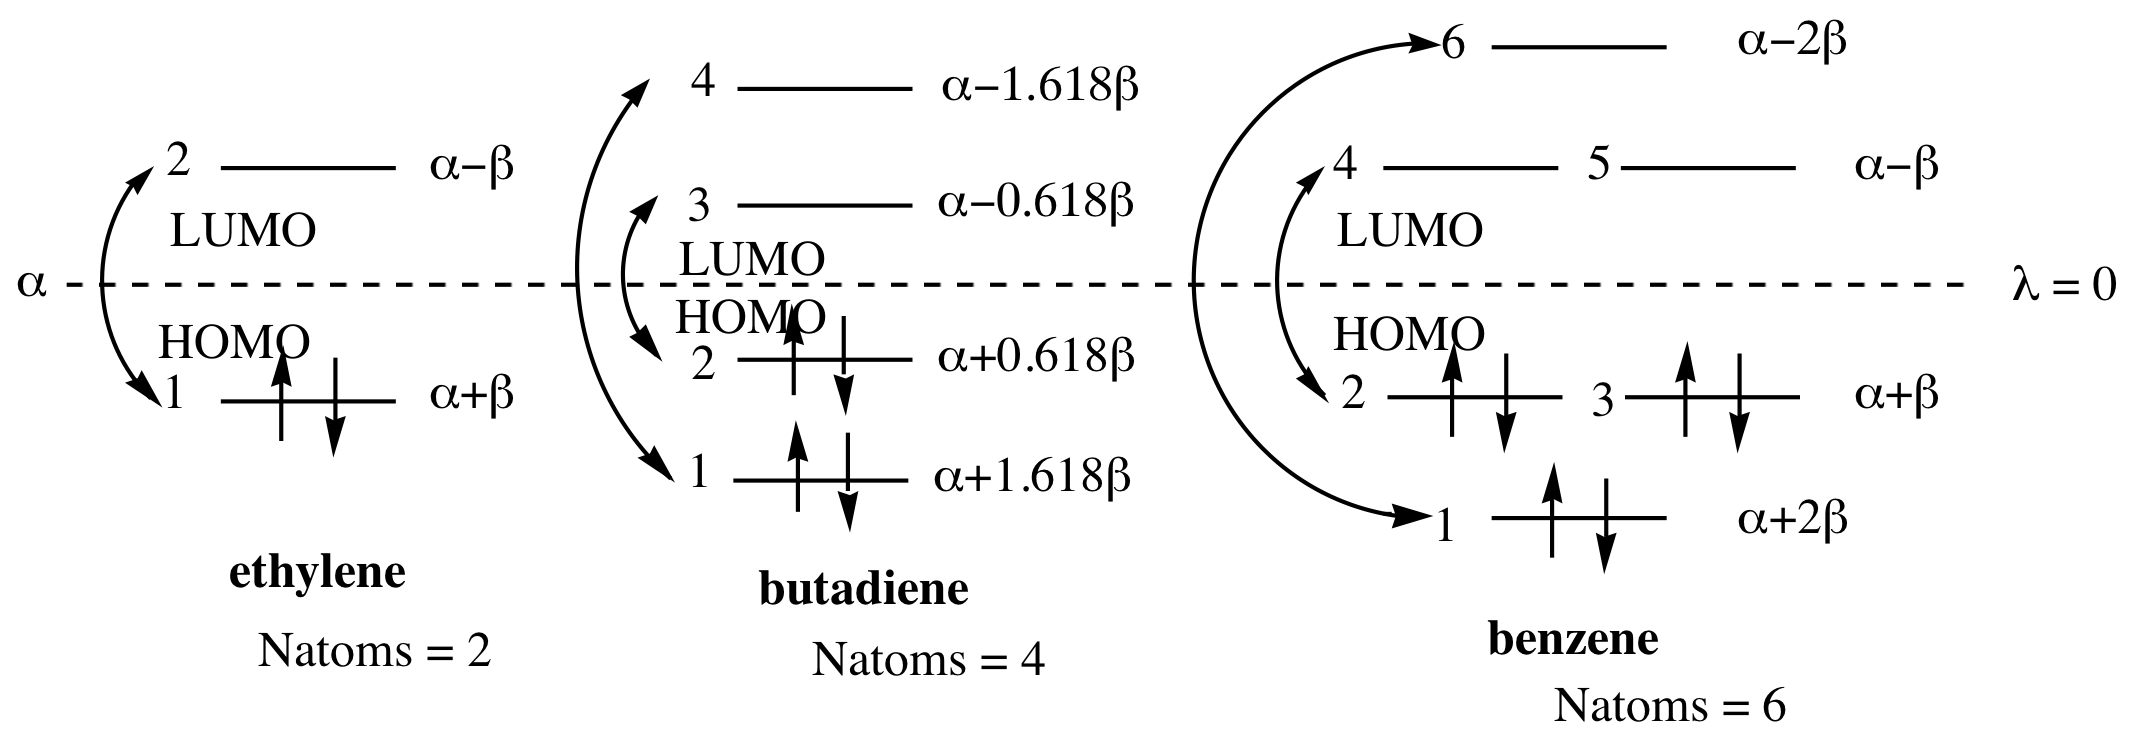
\includegraphics[width = 5in]{../huckel/c2_pairing_theorem.png}
\end{example}

An interesting implication is that alternant hydrocarbons with an odd number of carbons have an orbital with $\lambda_i = 0$, that is $\epsilon_i = \alpha$.
To see this consider the case $N = 2k + 1$ and consider the level $i = k + 1$. In this case the energy $\epsilon_{k + 1}$ is equal to that of $\epsilon_{N - (k + 1) + 1}$, from which we obtain
\begin{align}
\epsilon_{k + 1} = \epsilon_{N - (k + 1) + 1} \Rightarrow \alpha + \lambda_i \beta=  \alpha - \lambda_i \beta  \Rightarrow \lambda_i = 0.
\end{align}

\begin{example}[Pairing theorem for the allyl and benzyl radicals (odd alternant)]
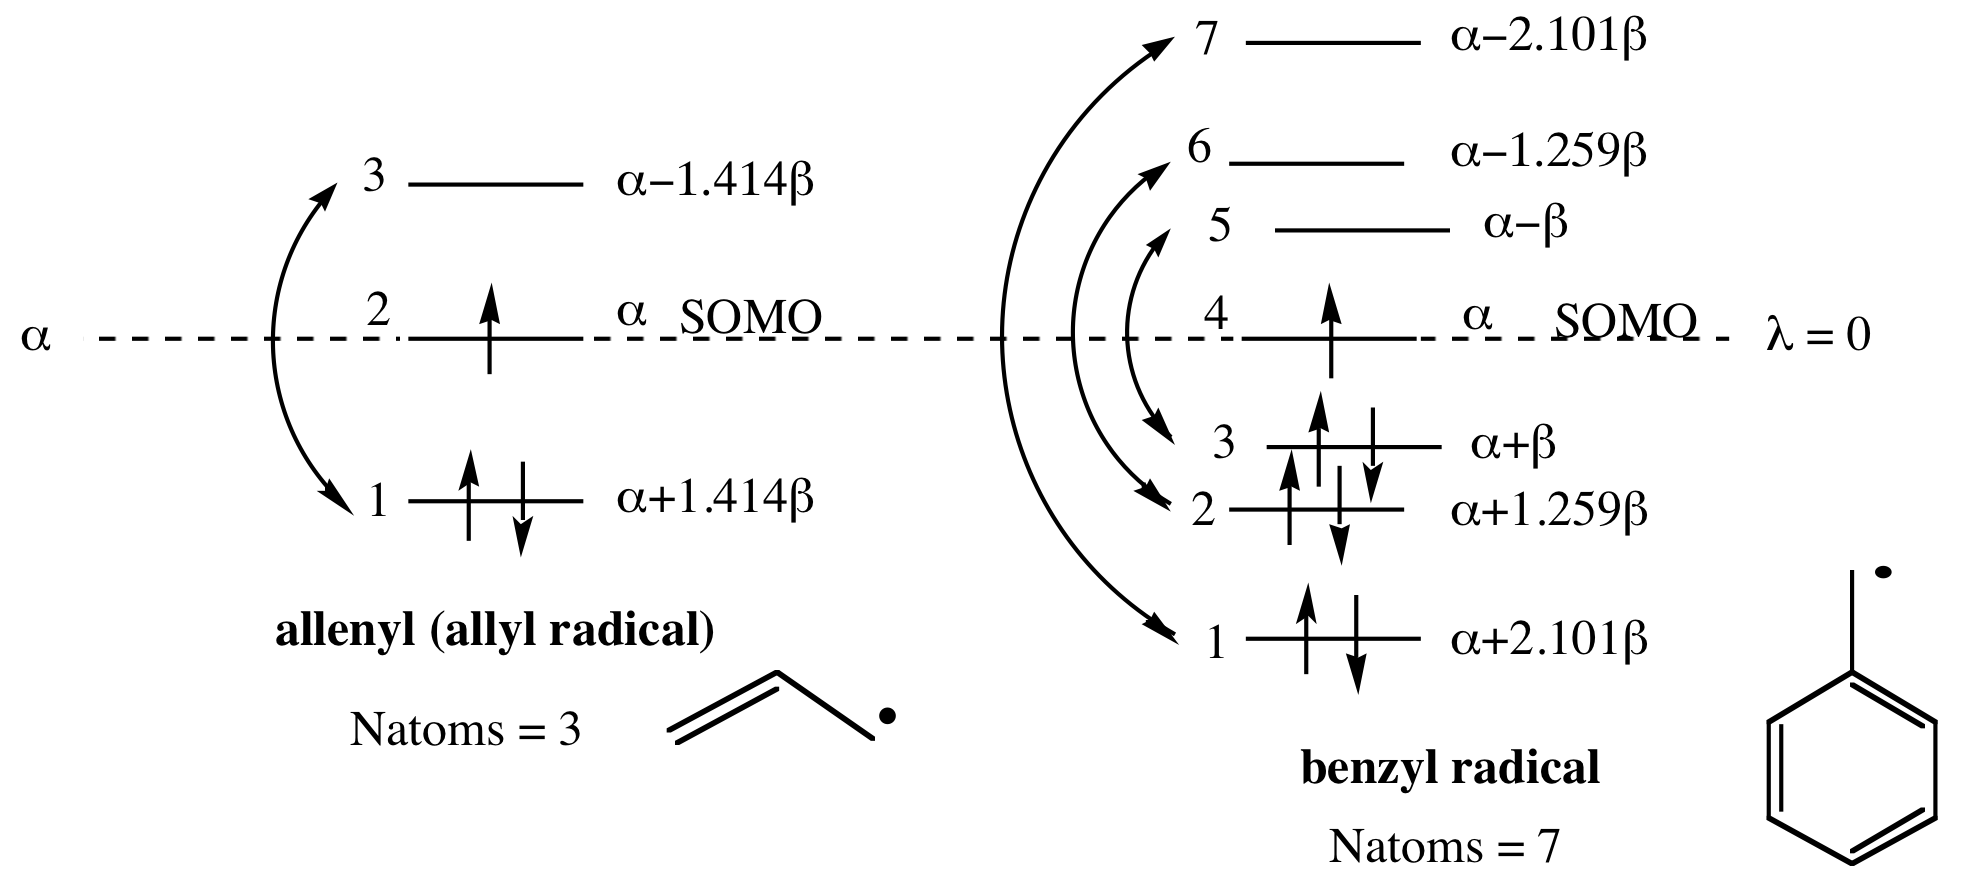
\includegraphics[width = 5in]{../huckel/c2_pairing_theorem2.png}

In the allyl radical the second MO ($\psi_2$, $\epsilon_2 = \alpha$) is paired to itself. In the benzyl radical the fourth MO ($\psi_4$, $\epsilon_4 = \alpha$) is paired to itself.
\end{example}

\begin{example}[Non alternant hydrocarbons]
In this example, the energies of the cyclopropenyl cation are not paired

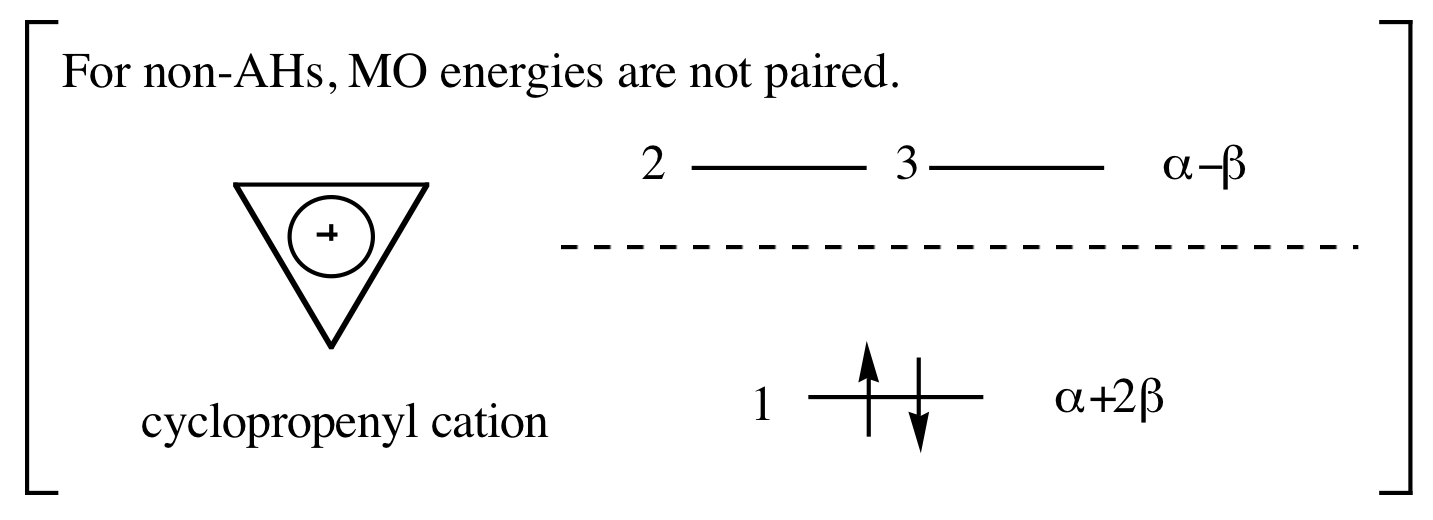
\includegraphics[width = 3in]{../huckel/c2_nonalternant.png}
\end{example}



Another consequence of this theorem is that the coefficients of paired orbitals are also paired (MOs $\psi_i$ and $\psi_{N-i+1}$ are paired). This property is best expressed by labeling alternating carbon atoms with a star (*) and the relationship
\begin{align}
C_{\mu, N - i + 1} &= \;\;\;C_{\mu i} \quad \text{ when $\mu$ = starred atom} \\
&= - C_{\mu i}  \quad \text{ when $\mu$ = unstarred atom}.
\end{align}

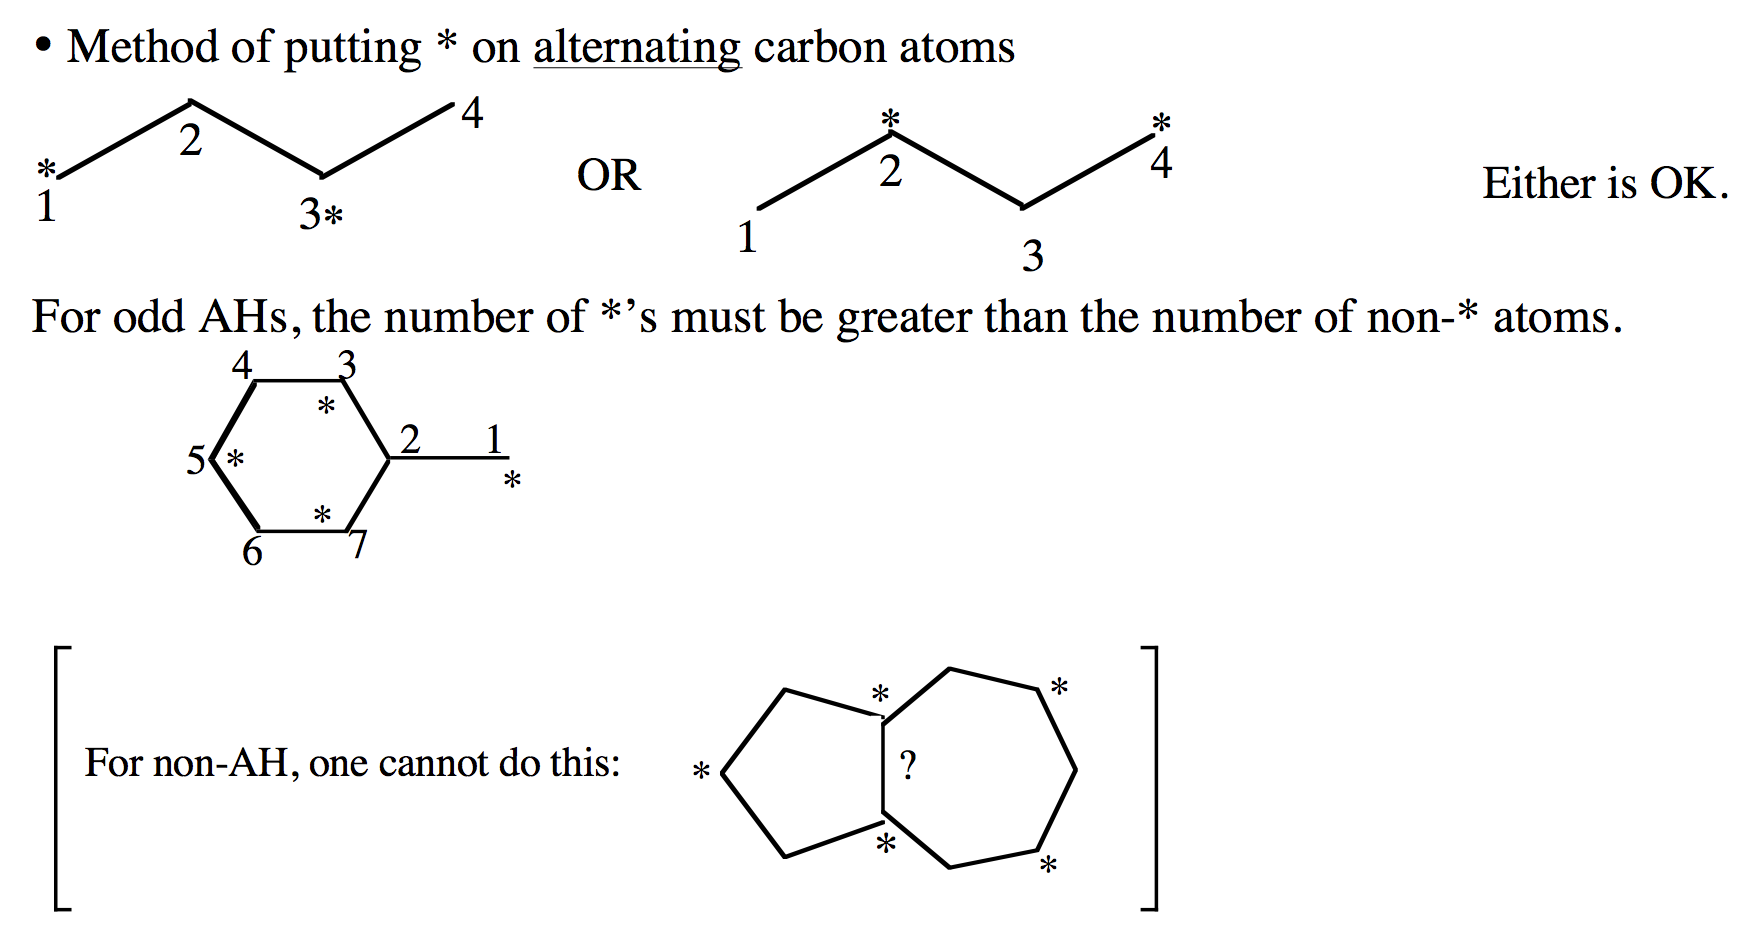
\includegraphics[width = 5in]{../huckel/c2_alternant.png}

\begin{example}[H\"{u}ckel computation on butadiene]
The following shows the energy and coefficient matrix for butadiene. 
\begin{verbatim}
 Energies
        1         2(HOMO)   3(LUMO)   4
       1.618034   .618034  -.618034 -1.618034    MO energies

MO coefficients
    0   .371748  -.601501   .601501  -.371748    <- AO1
    1   .601501  -.371748  -.371748   .601501    <- AO2
    2   .601501   .371748  -.371748  -.601501    <- AO3
    3   .371748   .601501   .601501   .371748    <- AO4
         MO1       MO2       MO3       MO4
\end{verbatim}
Note that the energies and coefficients of MOs 1 and 4 and MOs 2 and 3 are paired.
Do not forget that the sign of MO as a whole is arbitrary.  i.e. $\psi_i$ or $-\psi_i$ are both OK.
\end{example}

\begin{example}[H\"{u}ckel computation on allyl radical]
The following shows the energy and coefficient matrix for the allyl radical. 
\begin{verbatim}
 Energies
        1       2(SOMO)   3(LUMO) 
       1.414214 .000000 -1.414214    MO energies

MO coefficients
    0   -.500000 -.707107   .500000    <- AO1
    1   -.707107  .000000  -.707107    <- AO2
    2   -.500000  .707107   .500000    <- AO3
         MO1       MO2       MO3

DENSITY AND BOND ORDER MATRIX
         1        2         3 
    1   1.000000
    2    .707107 1.000000
    3    .000000  .707107  1.000000
         
DEGENERACIES: HOMO=0 LUMO = 0 TOTAL ENERGY = 3 ALPHA + 2.828427 BETA         
\end{verbatim}
Note that the energies and coefficients of MOs 1 and 3 are paired.
\end{example}

When MOs are degenerate (i.e., two MOs have same energy), their MO coefficients can not be uniquely determined.  Any linear combination of degenerate MOs is also acceptable MO of the same energy.  Appropriate transformation among degenerate MOs is needed to show pairing.

\begin{example}[H\"{u}ckel computation on benzene]
In this example, the MOs of the benzene molecule were transformed according to
\begin{align*}
\psi_2^\mathrm{new} & = +\cos \theta \psi_2 + \sin \theta \psi_3  \\
\psi_3^\mathrm{new} & = -\sin \theta \psi_2 + \cos \theta \psi_3 
\end{align*}
and chosen either to be such that $|C_{12}|$ is maximized, which in this case is also equivalent to $C_{13} = 0$.
\begin{verbatim}
 Energies
         1         2         3         4         5         6
        2.000000  1.000000  1.000000 -1.000000 -1.000000 -2.000000

 MO coefficients

    1   .408248   .455142   .355218   .567622  -.105541  -.408248
    2   .408248   .535198  -.216555  -.192409   .544345   .408248
    3   .408248   .080057  -.571773  -.375212  -.438804  -.408248
    4   .408248  -.455142  -.355218   .567622  -.105541   .408248
    5   .408248  -.535198   .216555  -.192409   .544345  -.408248
    6   .408248  -.080057   .571773  -.375212  -.438804   .408248
           1         2         3         4         5         6

 New Energies
        1         2         3         4         5         6
       2.000000  1.000000  1.000000 -1.000000 -1.000000 -2.000000

 New MO coefficients
    1   .408248   .577350   .000000   .577350   .000000  -.408248
    2   .408248   .288675  -.500000  -.288675   .500000   .408248
    3   .408248  -.288675  -.500000  -.288675  -.500000  -.408248
    4   .408248  -.577350   .000000   .577350   .000000   .408248
    5   .408248  -.288675   .500000  -.288675   .500000  -.408248
    6   .408248   .288675   .500000  -.288675  -.500000   .408248
           1         2         3         4         5         6

 DEGENERACIES:  HOMO=  2    LUMO=  2
\end{verbatim}
Shown above are two sets of orbitals for benzene. Note that orbitals 2 and 3 and 4 and 5 are degenerate. Therefore, we are allowed to separately mix them without changing the orbital energies.
\end{example}

\section{Symmetry of MOs}
Each MO is symmetric or antisymmetric with respect to symmetry operations of the system.

\begin{example}[Symmetry of the orbitals in butadiene]
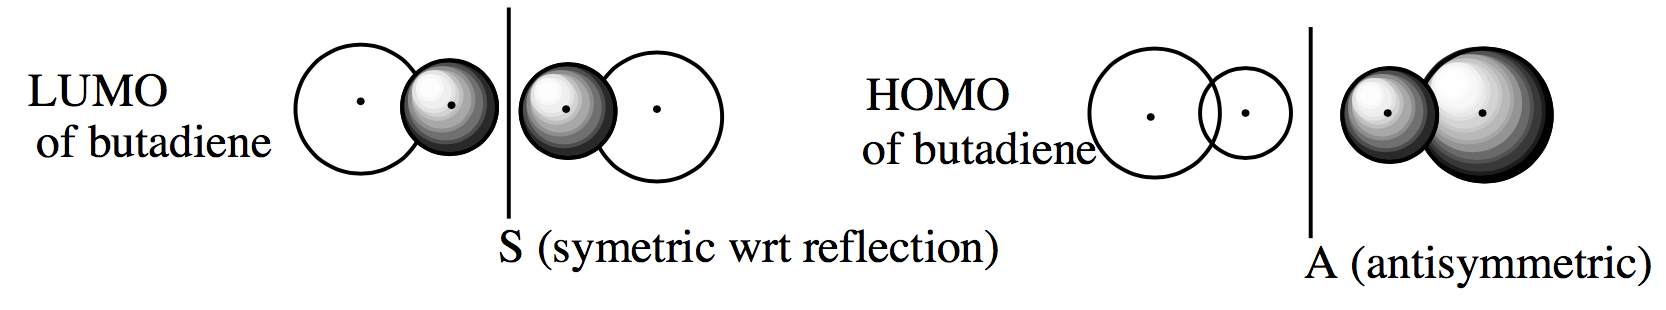
\includegraphics[width=4in]{../huckel/c2_symmetry_ex1.png}
\end{example}

\begin{example}[Symmetry of the orbitals in the allyl radical]
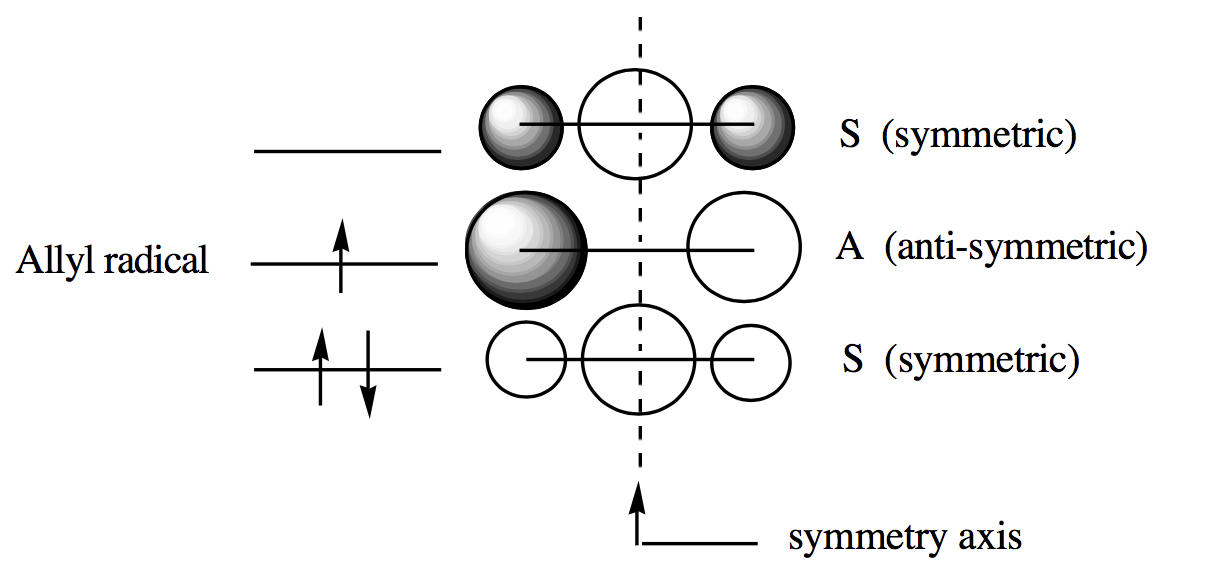
\includegraphics[width=3in]{../huckel/c2_symmetry_ex2.png}
\end{example}

\begin{example}[Symmetry of the orbitals in benzene]
This example shows that when MOs are degenerate, appropriate linear combinations of degenerate MOs can be made to satisfy symmetry.
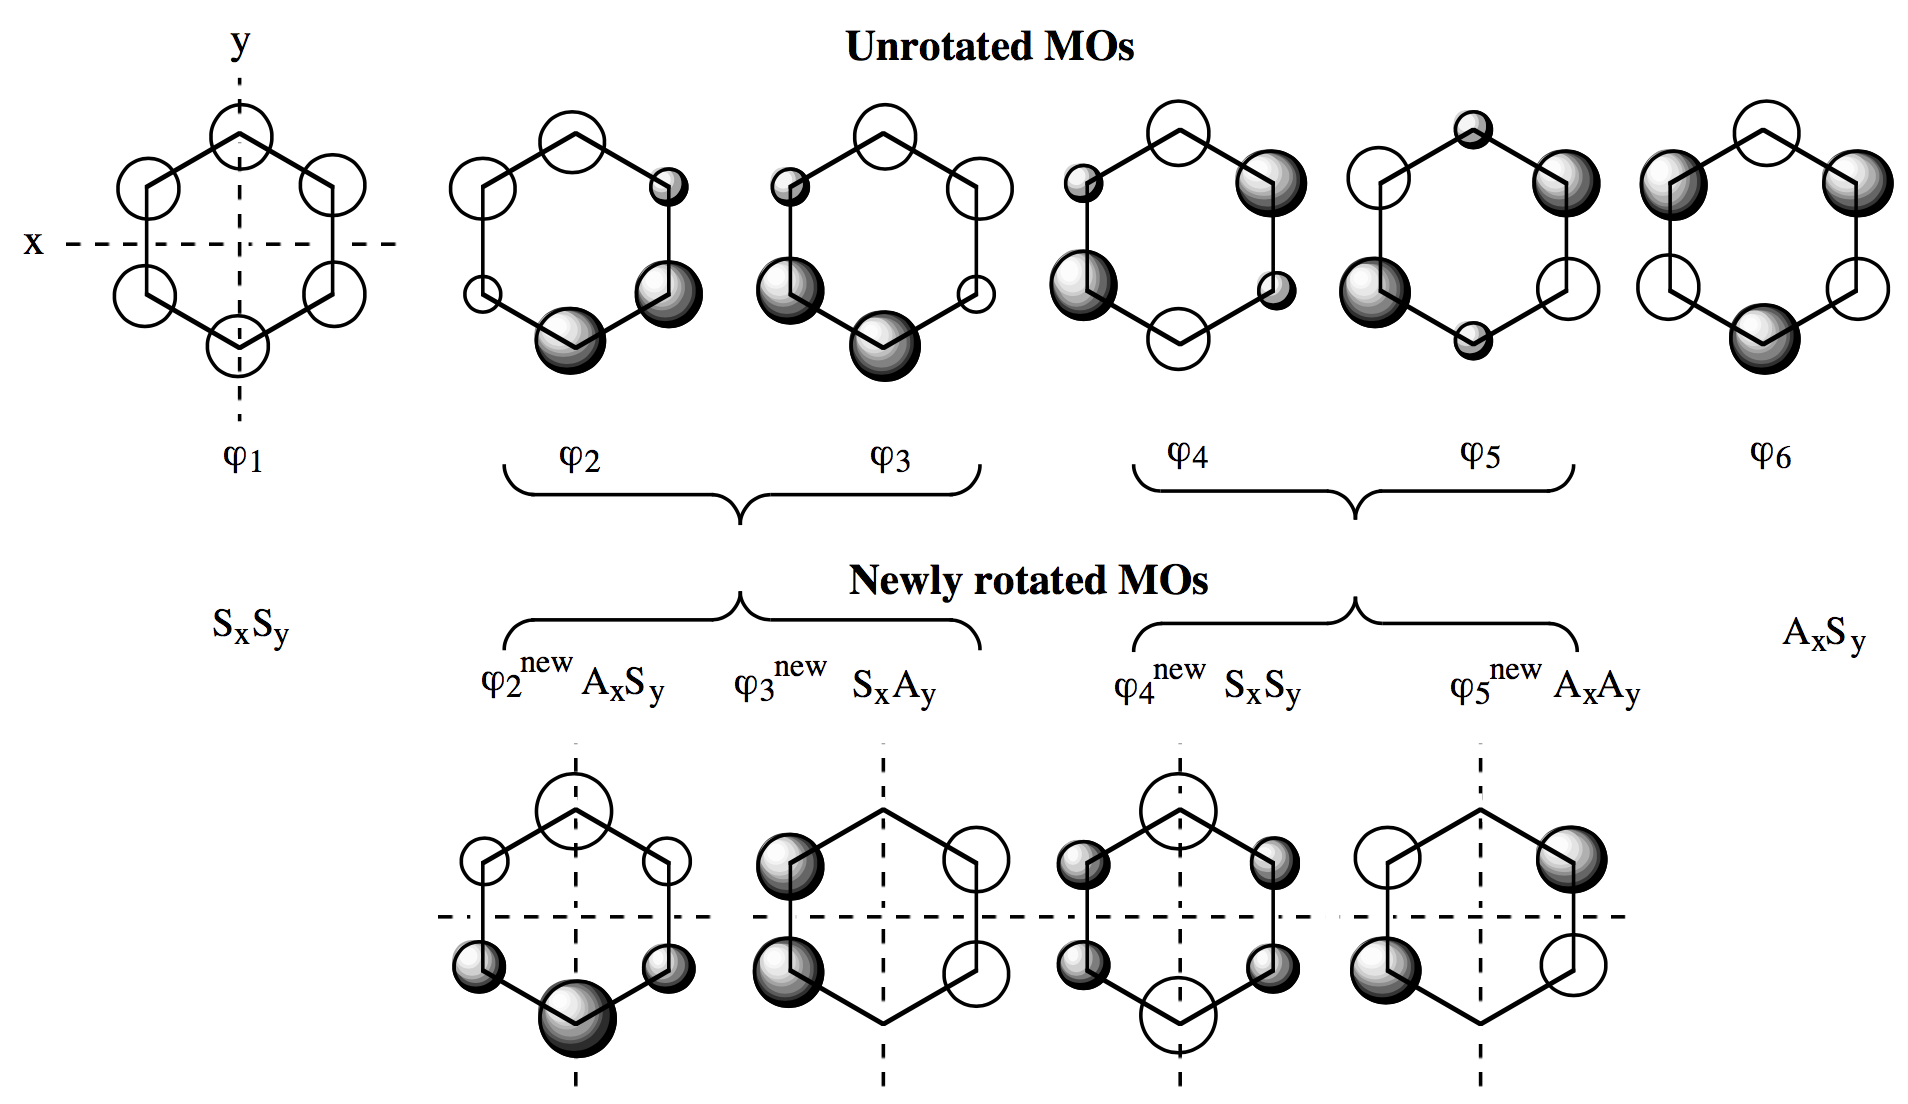
\includegraphics[width=4.5in]{../huckel/c2_symmetry_ex3.png}
\end{example}




\section{NBMO (Non-bonding MO) back-of-the-envelope calculation}

Once a wise man said: ``For odd alternant hydrocarbon radicals, the SOMO (Singly Occupied MO, $\lambda_i$=0) can be calculated by hand''.

This is a consequence of the pairing theorem for odd alternant hydrocarbon. Recall that the $\mu$-th row of the secular equation for the SOMO and $\mu$ = a non-starred atom is given by:
\begin{equation}
C_{\sigma_1 i} - \lambda_i C_{\mu i} + C_{\sigma_2 i} + C_{\sigma_3 i} = 0,
\quad 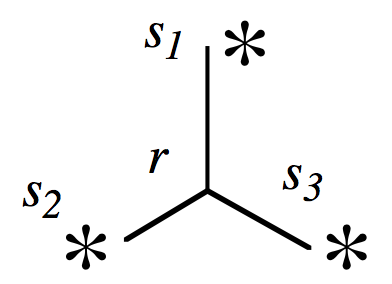
\includegraphics[width=1in]{../huckel/c2_nbmo_1.png}
\end{equation}
where $\sigma_j$ stands for a surrounding starred atom.
Since for the SOMO we have that $\lambda_i = 0$ then it follows that
\begin{equation}
\sum_{\sigma}^{\text{neighbors of non *atom}} C_{\sigma i} = 0.
\end{equation}

\begin{example}[Allyl radical]
For the allyl radical we can easily compute the SOMO

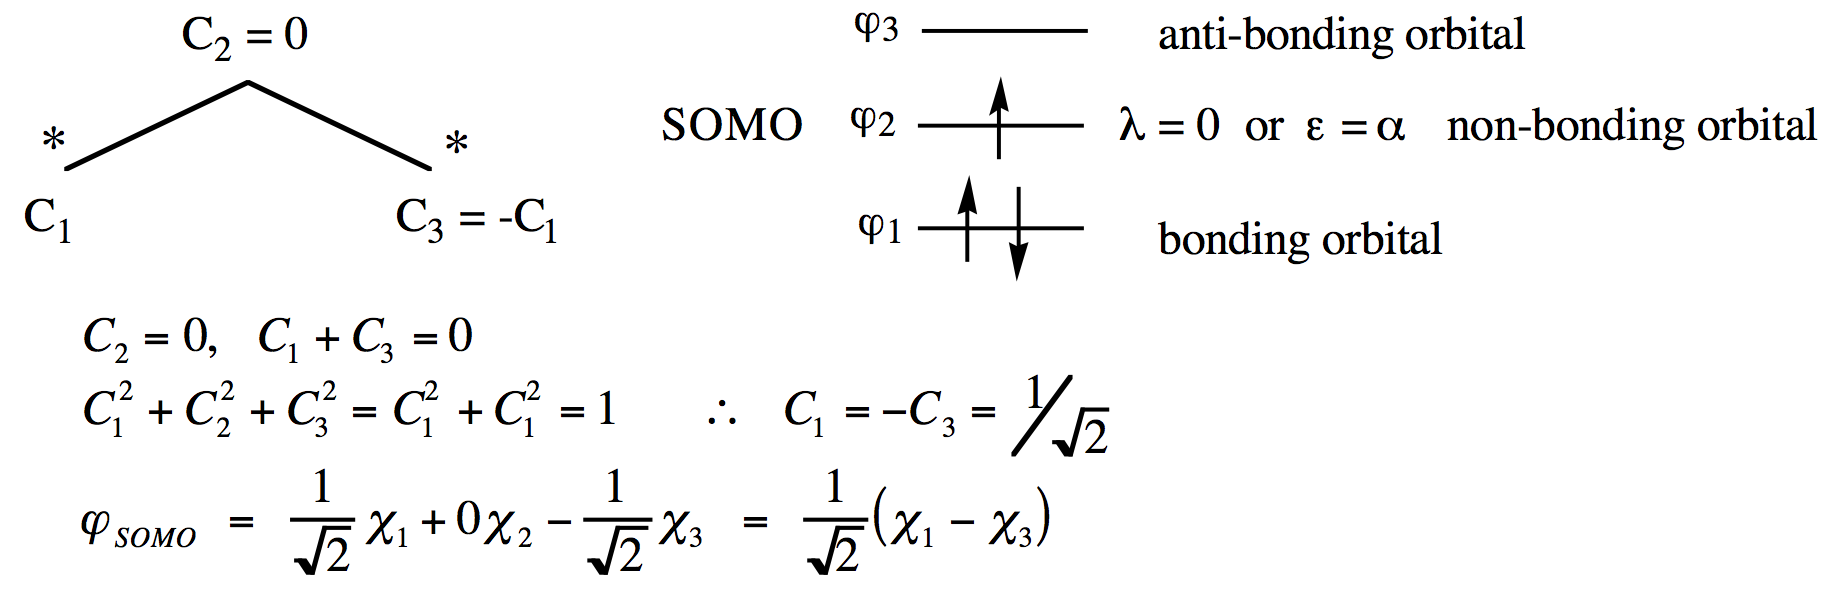
\includegraphics[width=4.5in]{../huckel/c2_nbmo_ex1.png}

\end{example}

\begin{example}[Benzyl radical] We can evaluate the reactivity

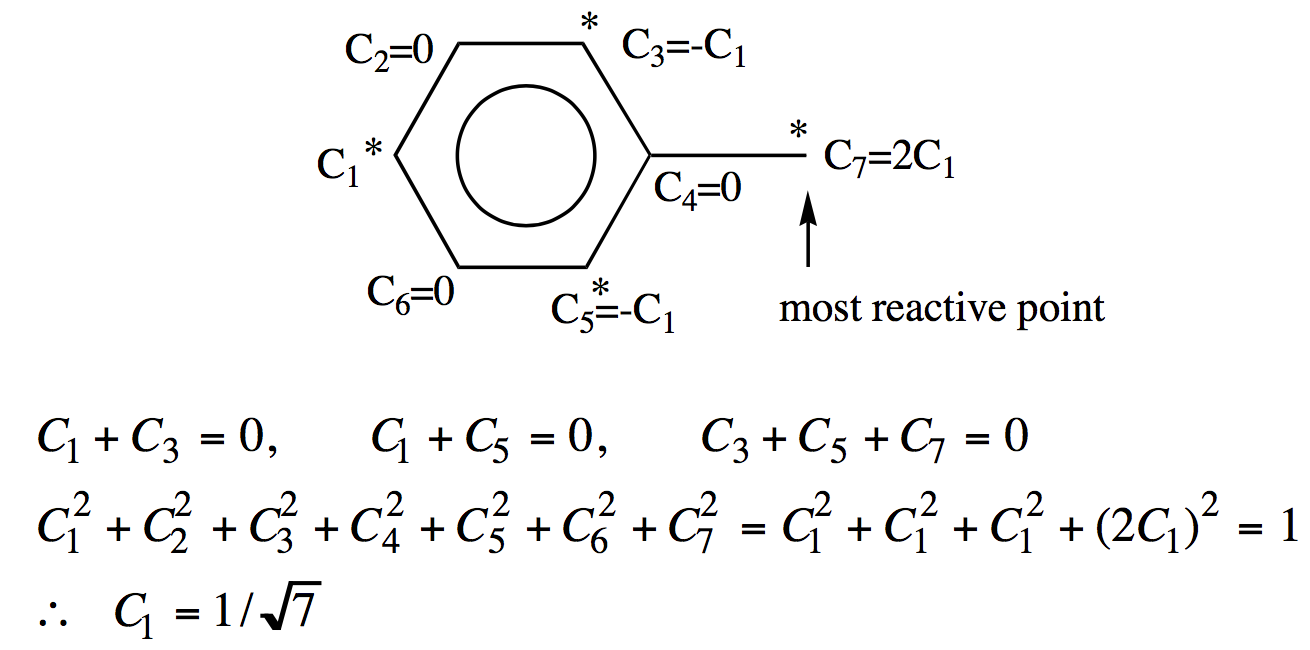
\includegraphics[width=3in]{../huckel/c2_nbmo_ex2.png}

\end{example}
	
What is this good for:
\begin{enumerate}
\item Showing off.
\item Predict the qualitative spin density distribution. (exp. measured by ESR)
\item Predict the qualitative reactivity of radicals.
\end{enumerate}

\begin{example}[Further examples] Consider the following molecules:

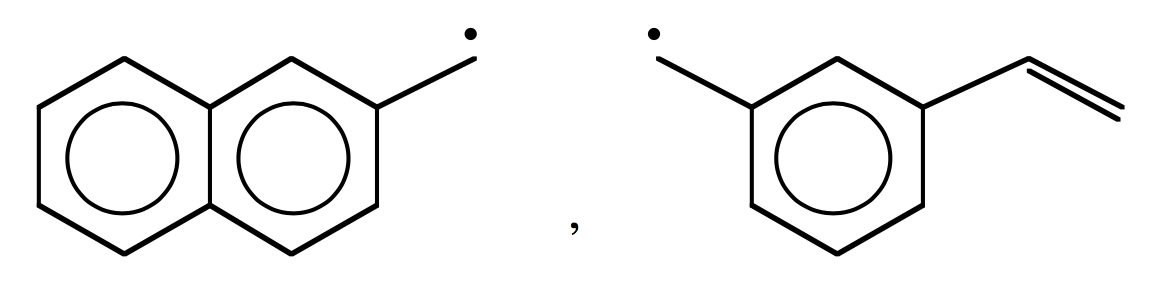
\includegraphics[width=3in]{../huckel/c2_nbmo_ex3.png}

\end{example}

\section{MO electron density and bond order, total electron density and total bond order}
Recall that $i$-th MO can be expanded in terms of the AOs ($\chi_\mu$ = AO) and the coefficient matrix ($C_{\mu i}$) as:
\begin{equation}
\psi_i = \sum_\mu^{N} \chi_\mu C_{\mu i}.
\end{equation}
Since each MO is normalized we can write:\mnote{Recall that in quantum mechanics $|\Psi|^2 = \Psi^* \Psi$ is a probability density.}
\begin{equation}
\begin{split}
1 = & \braket{\psi_i | \psi_i} = 
\sum_{\mu \nu}^N C_{\mu i}^*  \underbrace{\braket{\chi_\mu | \chi_\nu}}_{S_{\mu\nu}} C_{\nu i}
= \sum_{\mu}^N C_{\mu i}^* C_{\mu i}  S_{\mu\mu}
+ \sum_{\mu}^N \sum_{\substack{\nu\\ \nu \neq \mu}}^N C_{\mu i}^* C_{\nu i}  S_{\mu\nu} \\
= & \sum_{\mu} |C_{\mu i}|^2 + \sum_{\mu \neq \nu} C_{\mu i}^* C_{\nu i}  S_{\mu\nu}.
\end{split}
\end{equation}
\mnote{To simplify the notation we will write $\sum_{\mu} \sum_{\substack{\nu\\ \nu \neq \mu}}$ as $\sum_{\mu \neq \nu}$ and omit the superscript $N$.}
We can interpret the last two terms in the following way
\begin{itemize}
\item $q^i_\mu = |C_{\mu i}|^2$ is the probability of finding an electron in MO $\psi_i$ on the atomic orbital $\chi_\mu$. Therefore, we call this the \textbf{electron density} on AO $\chi_\mu$ due to the MO $\psi_i$.

\item $p_{\mu \nu}^i = C_{\mu i}^* C_{\nu i}$ may be interpreted as the \textbf{bond order} for bond $\mu$-$\nu$ in MO $\psi_i$ (recall that the H\"{u}ckel method assumes $S_{\mu\nu} = 0$ when $\mu \neq \nu$).
\end{itemize}

\begin{example}[Electron density for the first and second MOs of the allyl radical]

\begin{center}
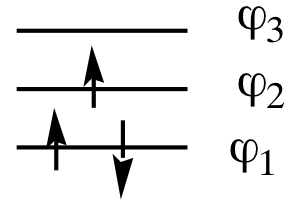
\includegraphics[width=1in]{../huckel/c2_allyl_ediagram.png}
\end{center}

For $\psi_1$
\begin{center}
\begin{tabular}{@{} lcr @{}} % Column formatting, @{} suppresses leading/trailing space
\toprule
AO & MO Coefficient ($C_{\mu i}$) & Electron density ($q^i_\mu = |C_{\mu i}|^2$)\\
\midrule
1 & $C_{11} = -0.5$ & $q_{1}^{1} = 0.25$ \\
2 & $C_{21} = -0.7071$ & $q_{2}^{1} = 0.5$ \\
3 & $C_{31} = -0.5$ & $q_{3}^{1} = 0.25$ \\
\midrule
Sum & & $\displaystyle \sum_{\mu = 1}^{N} q^1_\mu = 1.0$ \\
\bottomrule
\end{tabular}
\end{center}

For $\psi_2$
\begin{center}
\begin{tabular}{@{} lcr @{}} % Column formatting, @{} suppresses leading/trailing space
\toprule
AO & MO Coefficient ($C_{\mu i}$) & Electron density ($q^i_\mu = |C_{\mu i}|^2$)\\
\midrule
1 & $C_{12} = 0.7071$ & $q_{1}^{2} = 0.5$ \\
2 & $C_{22} = 0$ & $q_{2}^{2} = 0$ \\
3 & $C_{32} = -0.7071$ & $q_{3}^{2} = 0.5$ \\
\midrule
Sum & & $\displaystyle \sum_{\mu = 1}^{N} q^2_\mu = 1.0$ \\
\bottomrule
\end{tabular}
\end{center}
\end{example}


Using these quantities we define:
\begin{itemize}
\item \textbf{Total density on atom} $\mu$ ($q_\mu$):
\begin{equation}
q_\mu = \sum_{i}^{\rm MO} n_i |C_{\mu i}|^2 = \sum_{i}^{\rm MO} n_i q_\mu^i \quad n_i \text{ = occupation (2, 1, or 0)} 
\end{equation}

\item \textbf{Total charge on atom} $\mu$ ($N_\mu$):
\begin{equation}
N_\mu = (\text{number of $\pi$ electrons donated by atom $\mu$}) - q_\mu
\end{equation}

\item \textbf{Total bond order between atoms  $\mu$ and  $\nu$} ($p_{\mu \nu}$):
\begin{equation}
p_{\mu \nu}= \sum_{i}^{\rm MO} n_i C_{\mu i}^* C_{\nu i} = \sum_{i}^{\rm MO} n_i p_{\mu\nu}^i
\end{equation}
\end{itemize}

Note that the orbital energy may be rewritten using the orbital density ($q^i_\mu = |C_{\mu i}|^2$) and bond order ($p_{\mu \nu}^i = C_{\mu i}^* C_{\nu i}$)
\begin{equation}
\epsilon_i = \braket{\psi_i | \hat{h} | \psi_i} = \sum_{\mu} q_{\mu}^{i} \alpha_{\mu} + 2 \sum_{\mu <  \nu} p_{\mu \nu}^i \beta_{\mu\nu}.
\end{equation}
and the total energy can be also expressed using the total density and bond order as
\begin{equation}
E = \sum_i^\mathrm{occ} n_i \epsilon_i = \sum_{\mu} q_{\mu} \alpha_{\mu} + 2 \sum_{\mu < \nu} p_{\mu \nu} \beta_{\mu\nu}.
\end{equation}

\begin{example}[H\"{u}ckel computation on allyl radical]
The following shows the density and bond order matrix for the allyl radical. 
\begin{verbatim}
Density and bond order matrix
         1         2         3 
    1   1.000000  0.707107  0.000000
    2   0.707107  1.000000  0.707107
    3   0.000000  0.707107  1.000000
\end{verbatim}

\begin{center}
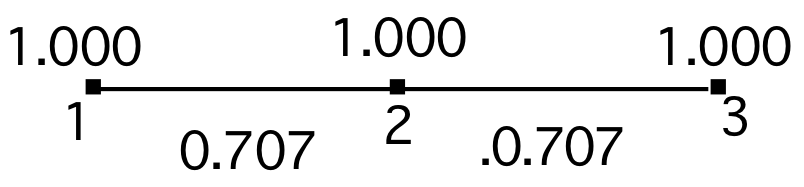
\includegraphics[width=2in]{../huckel/c2_allyl_bond_order.png}
\end{center}

\begin{equation}
p_{12} = 2 C_{11} C_{21} +  C_{12} C_{22} = 2 \times 0.5 \times (-0.7071) + 0.7071 \times 0 = 0.7071.
\end{equation}

Note that for alternant hydrocarbons the pairing theorem always gives $q_\mu = 1$.
\end{example}

\begin{example}[H\"{u}ckel computation on butadiene]
The following shows the density and bond order matrix for butadiene. 
\begin{verbatim}
Density and bond order matrix
         1         2         3         4 
    1   1.000000  0.894427  0.000000 -0.447214
    2   0.894427  1.000000  0.447214  0.000000
    3   0.000000  0.447214  1.000000  0.894427
    4  -0.447214  0.000000  0.894427  1.000000
\end{verbatim}

Note that the 1-2 and 3-4 bonds ($p_{12} = p_{34} = 0.894427$) are stronger than the 2-3 bond ($p_{23} = 0.447214$). Also, ignore the negative values for non-nearneighbor atoms.
\end{example}

\begin{example}[H\"{u}ckel computation on pyridine]
The following shows a full H\"{u}ckel computation for pyridine. 
\begin{verbatim}
 NATOMS  NELECS  NINDEX   NLAB   NHOMO   NLUMO
    6       6       0       1       3       4

 Input Matrix
       1       2       3       4       5       6
    1   .5000
    2  1.1000   .0000
    3   .0000  1.0000   .0000
    4   .0000   .0000  1.0000   .0000
    5   .0000   .0000   .0000  1.0000   .0000
    6  1.1000   .0000   .0000   .0000  1.0000   .0000

 Energies
    1         2         3         4         5         6
   2.199322  1.206641  1.000000  -.916933 -1.000000 -1.989029
 
 MO coefficients 
    1   .558416   .525891   .000000   .528265   .000000  -.364069
    2   .431331   .168916   .500000  -.340234   .500000   .411900
    3   .334378  -.374659   .500000  -.269119  -.500000  -.418804
    4   .304074  -.620995   .000000   .586999   .000000   .421114
    5   .334378  -.374659  -.500000  -.269119   .500000  -.418804
    6   .431331   .168916  -.500000  -.340234  -.500000   .411900
    
 Total energy = 6 ALPHA +  8.811924 BETA

 Density and bond-order matrix
        1          2         3         4         5         6
    1  1.176780 
    2  0.659388   0.929159
    3 -0.020615   0.661883  1.004356
    4 -0.313552   0.052521  0.668674  0.956191
    5 -0.020615  -0.338117  0.004356  0.668674  1.004356
    6  0.659388  -0.070841  -.338117  0.052521  0.661883  0.929159

 Total charges:
	N1: 1 - 1.177= -0.177
	C2: 1 - 0.929= +0.071
	C3: 1 - 1.004= -0.104
	C4: 1 - 0.956= +0.044
\end{verbatim}
\end{example}

\begin{example}[H\"{u}ckel computation on pyrrole]
The following shows a full H\"{u}ckel computation for pyrrole. 
\begin{verbatim}
NATOMS  NELECS  NINDEX   NLAB   NHOMO   NLUMO
    5       6       0       1       3       4

 Input Matrix
       1       2       3       4       5
    1   .8000
    2   .9000   .0000
    3   .0000  1.0000   .0000
    4   .0000   .0000  1.0000   .0000
    5   .9000   .0000   .0000  1.0000   .0000

 Energies
         1         2         3         4         5
       2.120048   .920296   .618034 -1.240344 -1.618034

 MO coefficients
    1  -.583903  -.643479   .000000   .494968   .000000
    2  -.428211  -.043004  -.601501  -.561058  -.371748
    3  -.382315   .539554  -.371748   .250434   .601501
    4  -.382315   .539554   .371748   .250434  -.601501
    5  -.428211  -.043004   .601501  -.561058   .371748

 Total energy = 6 ALPHA +  7.316756 BETA

 Density and bond-order matrix
          1         2         3         4         5
    1  1.510014
    2   .555412  1.094034
    3  -.247914   .728230  1.150959
    4  -.247914  -.166198   .598172  1.150959
    5   .555412  -.353179  -.166198   .728230  1.094034

 Total charges:
    N1: 2 - 1.510= +0.490
    C2: 1 - 1.094= -0.094
    C3: 1 - 1.151= -0.151
\end{verbatim}
\end{example}

\end{document}